
\chapter{Introduction}
\label{Chap:Intro}

This thesis considers the problem of tracking human wrist movements during free living.
The goal is to build a device that can track these movements continuously all day,
storing the data so that it can be processed later.
While many wrist-worn devices with tracking capabilities are manufactured for the commercial and research markets, none has specifically addressed the need of recording translational and rotational wrist motion for an extended period of time.  Many devices do not include the necessary sensors to track rotational motion, or include unneeded features that make the device larger than necessary and require frequent recharging.
Device cost is also a factor given the desire to record data for many subjects over extended periods of time.
The work in this thesis was motivated by the goal of designing and prototyping a device that limits functionality to the goal of tracking and recording wrist motion all day while minimizing device size and cost.

The technical challenges of the problem are motivated by the size and power usage of the required components.
The sensors necessary for tracking wrist motion are a 3-axis accelerometer and a 3-axis gyroscope.
At the time of this writing, both types of sensors are available in small microelectricalmechanical systems (MEMS) packages with chip dimensions only a few millimeters.
Thus, they can be comfortably worn in a wrist-mounted package.
However, their power consumption varies by an order of magnitude.  MEMS accelerometers typically draw a current in the range of 300-500 $\mu$A and MEMS gyroscopes typically draw 3-10 mA of current.
To be worn on a wrist, these sensors must be powered by a battery.
Common small batteries used in wrist based devices have a capacity of 20-200 mAh.
These capacities allow for the continuous operation of a MEMS accelerometer for up to a week on a single charge.
However, a MEMS gyroscope
could typically operate for only 5-15 hours on a single charge.
The battery size is particularly important because it is usually the largest part in the device.
Since the goal is to mount the device on the wrist,
we are motivated to keep the battery size as small as possible.
These technical challenges are confounded if other unnecessary parts are included in the device.


\section{Motivation}
\label{Sec:Motivation}

The motivating vision for this work is a wrist mounted device that trackings wrist motion to detect when a person is eating,
counting the number of bites consumed in each meal.
In previous research our group has demonstrated algorithms where periods of eating can be detected with 81\% accuracy \cite{Dong2014},
and the number of bites in these meals can be counted with 86\% accuracy \cite{Dong2012}.
To further this research,
a device is needed that will facilitate the recording of wrist motion data for a large number of subjects, preferably with each subject recording for several days or even weeks.  This data could then be used to improve the detection and measurement algorithms.

For example, our previous work has suggested that the gyroscopes may not need to be powered continuously to detect periods of eating \cite{Dong2014}.  Instead, accelerometers could be powered continuously with gyroscopes only powered during periods of suspected eating to determine a final classification \cite{Dong2014}.  To test this idea, a large data set of continuous full wrist motion needs to be recorded.  Algorithms that processed the gyroscope data at intermittent intervals could be compared to algorithms that processed all the gyroscope data.

As another example, algorithms could be custom calibrated to an individual, perhaps improving performance over algorithms that are only tuned to the group level.  This is only feasible if sufficient data is recorded per person to enable custom tuning of thresholds or other algorithm parameters.  To facilitate collecting this amount of data, a device that is comfortable to wear for many days is necessary in order to encourage enough subjects to collect the necessary data.
 

\section{Existing devices}
\label{Sec:FitnessTracking}

Table \ref{Tab:IntroComp} shows a list of some devices on the market that can be used to track wrist motion and could potentially be used for the envisioned work.
There are four main categories.  The first category is fitness trackers.  It includes devices like the
Fitbit \cite{Web:FitBitOfficial} and Jawbone \cite{Web:JawBoneWebsite} series of sensors.
\inputfile{IntroCompTable.tex}
These devices allow for exercise and sleep monitoring. The Fibit activity monitor can be seen in figure \ref{fig:FitbitJawbone}~\cite{Web:FitbitImage}.  Its data is sent to a computer or a mobile phone to be viewed graphically by the user.
Many of these devices can be worn the wrist, are small, relatively low-cost, and can be powered for a week or longer on a single battery charge.
However, they do not include gyroscopes.  Activity monitoring is accomplished solely through the use of accelerometers.  In addition, accelerometer data is not stored continuously.  Instead, 10-60 second windows of data are reduced to single measurements that are related to step count, physical activity, or sleep activity, by on board processing of the raw sensor data.    Thus, none of these devices are designed to sense or record continuous wrist motion data.

\begin{figure}
\begin{center}
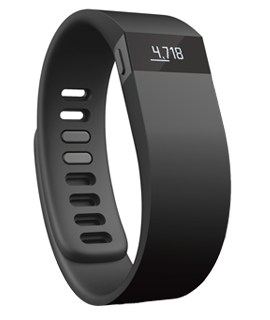
\includegraphics[width=0.4\textwidth]{images/JawFit.png}
\caption{The Fitbit flex activity tracker.}
\label{fig:FitbitJawbone}
\end{center}
\end{figure}

Another relevant class of devices is smart phones.  These devices commonly include gyroscopes and can be custom programmed to sense and record data continuously.  They contain larger batteries than fitness monitors, and so can power gyroscopes for more than 10 hours.  They also contain large memories that can store the raw sensor data for an extended period of time.  In our group's preliminary work, an Apple iPhone was used to record data from 44 subjects for a single day each \cite{Dong2014}.  However, smart phones are large and not intended to be worn on the wrist.  The comfort level of participants was lower than desired.  Smart phones are also relatively expensive.

A third class of devices that has recently emerged is the smart watch.  Examples include the Pebble and Samsung Gear.  These devices include many parts common to smart phones and are packaged in a wrist-worn assembly.  The goal is to enable viewing of text messages and other data commonly viewed on a smart phone on a smaller screen worn on the wrist.  A smart watch typically uses low power Bluetooth to communicate with a paired smart phone.  Some of these devices include gyroscopes and most can be custom programmed.  However, they are relatively larger than fitness devices due to their inclusion of a large display, wireless connectivity, and other features typically associated with smart phones.  They are also relatively expensive.

A fourth class of relevant devices are those produced for research use.  Examples include devices produced by XSens and Shimmer labs.  These devices provide generic tracking capabilities.  They are generally intended to be positioned or worn anywhere, so few specialize in wrist-mounted packaging.  While they can include gyroscopes and facilitate custom programming, they also serve wide markets and thus tend to include parts and capabilities not necessary for the goal of this work.  This tends to increase size and expense.


\section{Novelty}
\label{Sec:WearbleTracker}

The purpose of this work is to design and prototype a device that targets the goal of tracking and recording wrist motion continuously for a day.  The challenges are to meet or surpass the existing devices listed in Table \ref{Tab:IntroComp} in terms of the collective listed criteria.  Towards that goal, this thesis describes an investigation of the parts currently available for use in building such a device, including sensors, memory, batteries, connectors, and materials and methods used for embedded device construction.  After selecting parts and an overall design, a functioning prototype device was consructed.  Its operating characteristics are compared to the devices listed in table \ref{Tab:DevCompare} at the end of this thesis.

